\documentclass[12pt]{article}
%\usepackage[a4paper, total={6.5in, 8in}]{geometry}
\usepackage{graphicx}  % Add graphics capabilities
 \usepackage{color}

\usepackage{amsmath} % assumes amsmath package installed
\usepackage{amssymb}  % assumes amsmath package installed
\usepackage{amsthm}
\usepackage{epstopdf}
\usepackage{float}

\title{\LARGE \bf Discussion of CERN Objectives}
\begin{document}
\maketitle

\hrule
\begin{flushright}
Date: 27/06/2016
\end{flushright}
\textbf{Discussion 1: Optimal gains for voltage loop}

We are now trying to design controllers for the inner-loop of the power converter control system. Upper management has insisted that they want to control the inner loop with gains only. We are able to analytically derive the solutions for the gains such that a desired bandwidth is achieved, but there are some limitations to the amount of bandwidth that you ask for. 

We know that for bandwidths of less that $100 \: Hz$, the analytical solution gives us very goods results. I am now trying to use the data-driven method to obtain the solution for the gains, but the resulting solution from the optimization problem does not give good results. To obtain the gains, I am using the $H_\infty$ weighted sensitivity method. The closed-loop transfer function is given as follows:
\begin{equation}
T(s) = \frac{k_wG(s)}{1+k_iG(s)H(s) + k_uG(s)}
\end{equation} 
where $k_i, k_u, k_w$ are the gains to be found. $G(s)$ and $H(s)$ are stable transfer functions ($G$ is strictly proper, $H$ is proper, $H^{-1}$ is marginally stable). The sensitivity function that I shaped is:
\begin{equation}
S = 1-T =\frac{1+k_iGH+G(k_u-k_w)}{1+k_iGH+k_uG} 
\end{equation}
What is nice is that the numerators and denominators of these sensitivity functions are linearly parameterized in the gains, so the SPR condition can be used to formulate the convex optimization problem for $\| W_1S\|_\infty < \gamma$:
\begin{equation}
\Re \{ 1+k_iGH+k_uG\} > \gamma^{-1} |W_1(1+k_iGH+G(k_u-k_w))| 
\end{equation}
where $W_1 = (1-T_{des})^{-1}$ and $T_{des}$ is the desired closed loop transfer function. We have been selecting $T_{des}$ as a typical second order damped transfer function ($T_{des} = \omega_n^2(s^2+2\zeta\omega_n s + \omega_n^2 )^{-1}$). For $\zeta = 0.8$ and a desired bandwidth of $100 \: Hz$, the analytical solution produces satisfactory results; but the convex optimization problem does not produce gains that give good results. In fact, I get $\gamma_{opt} = 32.5$. Fig.~\ref{fig:volt_comp} shows the FRF comparison between the responses obtained.
\begin{figure}
\centering
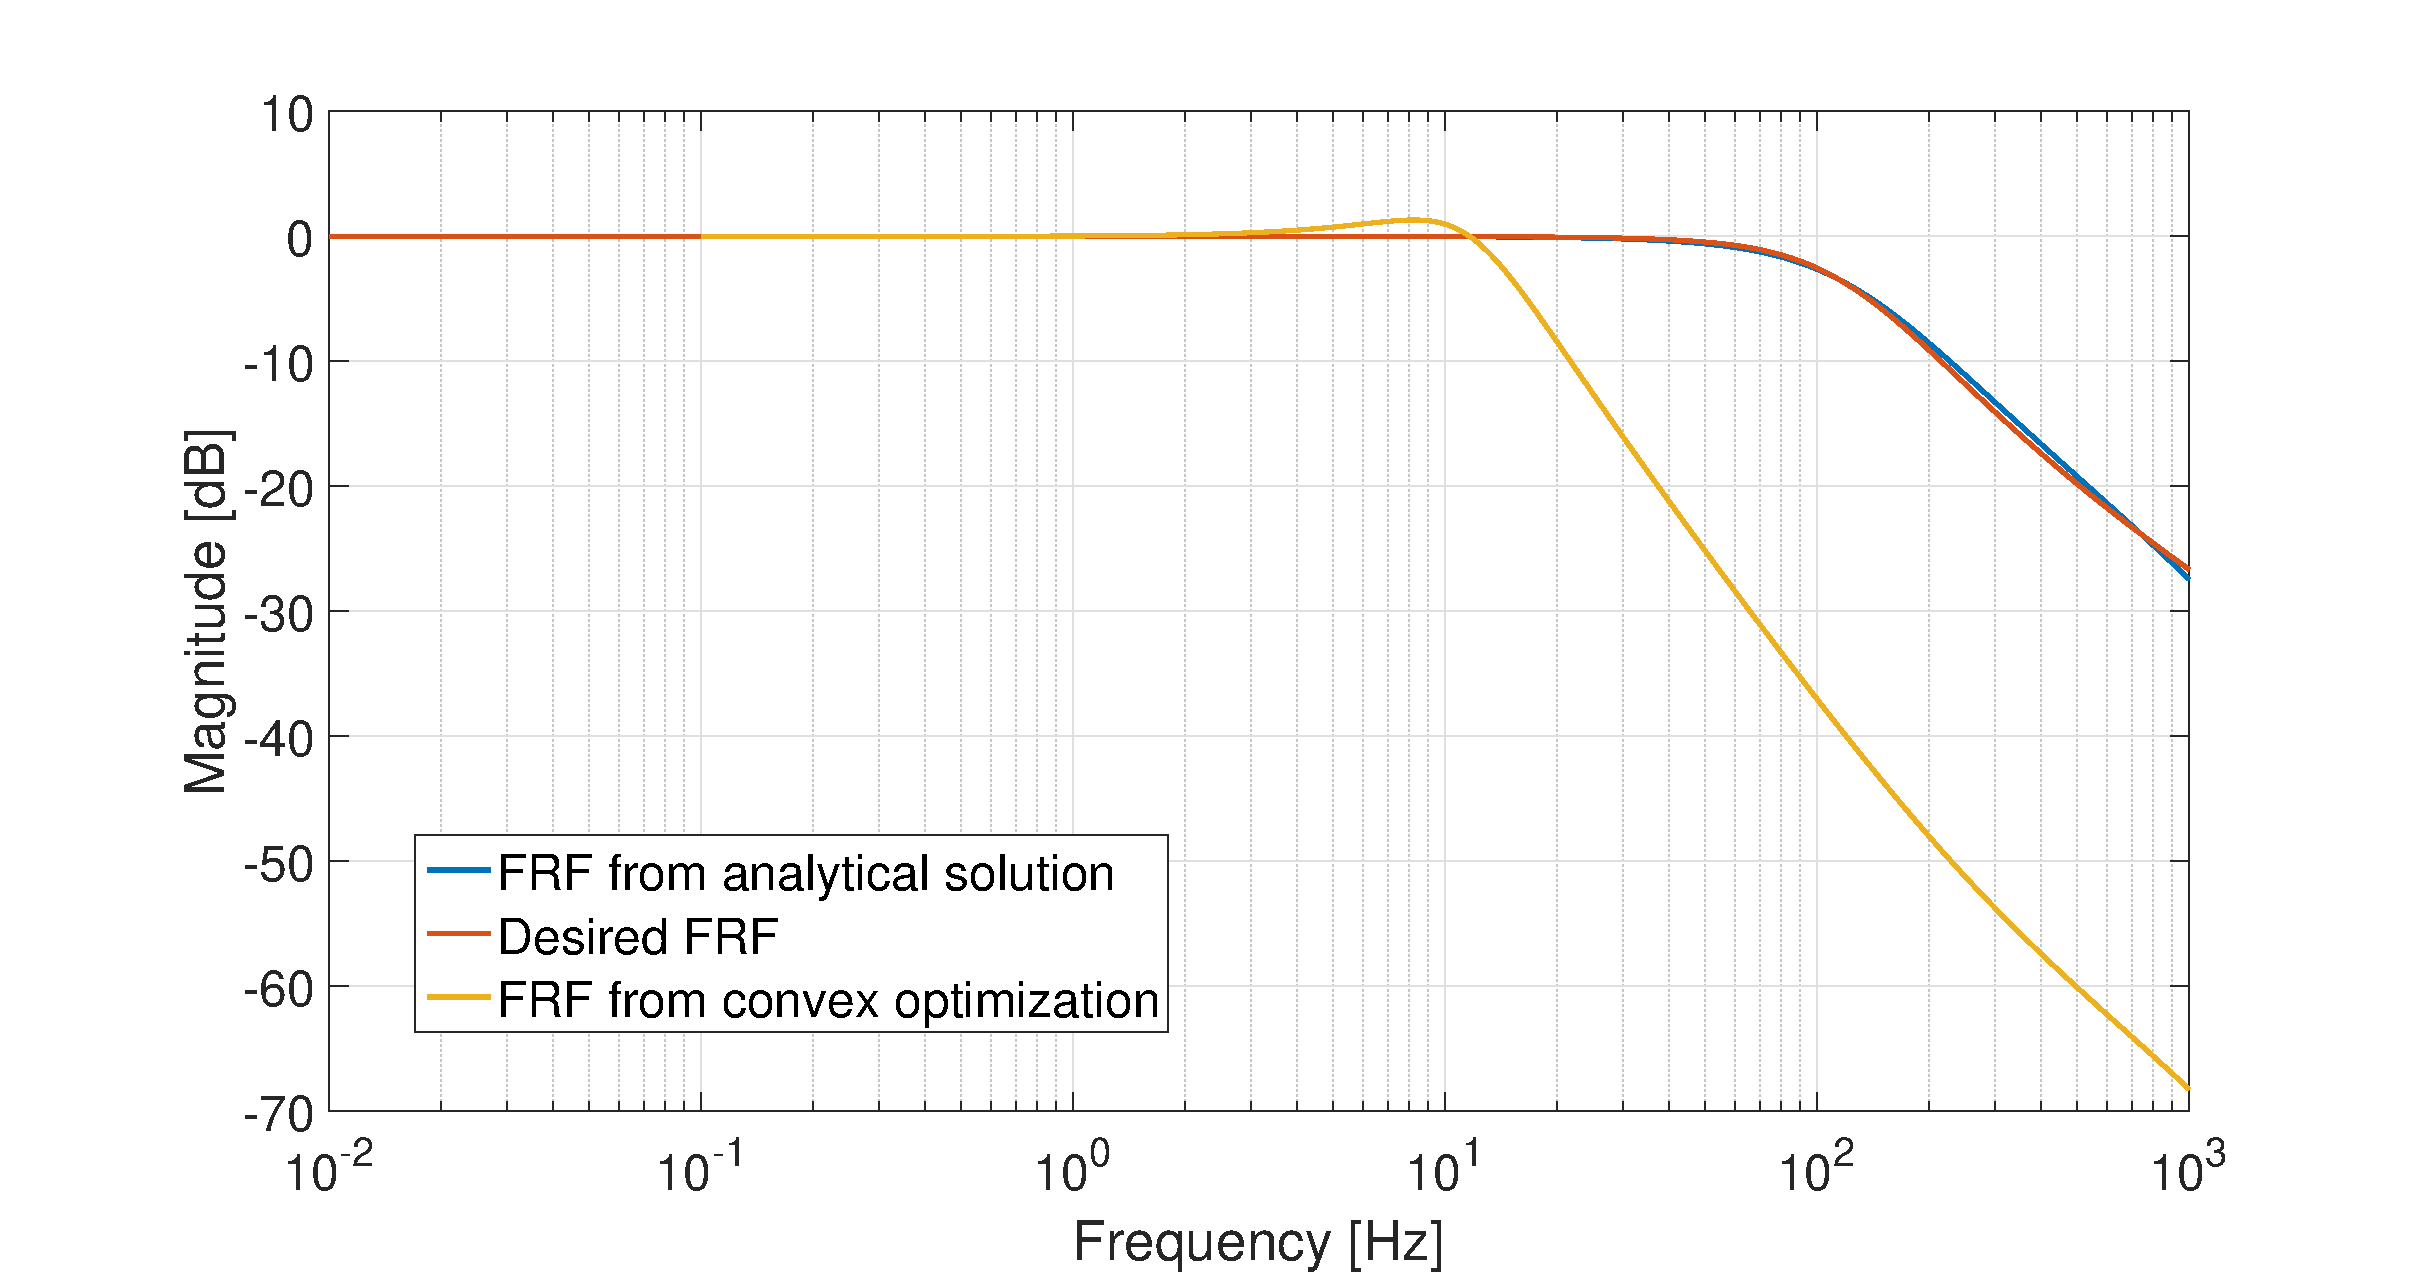
\includegraphics[width=\columnwidth]{pics/voltage_loop.eps}
\caption{Closed-loop FRF comparison between solutions obtained.}
\label{fig:volt_comp}
\end{figure}

What do you think the issue is? Am I shaping the wrong sensitivity function? Is there a limitation with the $H_\infty$ method by using strict gains? 

{\bf Answer AK:} The convexification for fixed low order controllers is too conservative. In fact there exists a multiplier F that reduces the conservatism but make the problem non-convex (that can be solved by PSO).

Another solution is to use the linearization method that I sent you sometimes ago by H2 control, which I believe has less conservatism for your problem. The similar linearization can be used also for H infinity if you wish.

{\bf Answer AN:} I will now attempt to derive the convex optimization problem (using the Shur complement lemma) for the specific controller configuration that we have for the damping loop. Below is a figure of the damping loop, where it is desired to find the gains $k_i$ and $k_u$ such that the desired bandwidth (with desired damping) is achieved. 
\begin{figure}
\centering
\resizebox{1\columnwidth}{!}{\input{damping_loop.pdf_tex}}
\caption{Damping loop}
%\label{fig:pc}
\label{fig:damping_loop}
\end{figure}

The closed-loop TF is:
\begin{equation}
T(s) = \frac{(1+k_u)G(s)}{1+k_iG(s)H(s) + k_uG(s)}
\end{equation} 
The error sensitivity function will be:
\begin{equation}
S =1-T =  \frac{1+k_iGH - G}{1+k_iGH + k_uG}
\end{equation} 
Using the sufficient condition you present in your paper with Christoph, we can formulate the loop-shaping constraint. But instead of shaping the open-loop TF $L(s)$, we can shape the closed-loop TF directly. In the $H_\infty$ sense, the optimization problem to solve is:
\begin{equation} \label{eq:min_loopshape}
\begin{aligned}
& {\text{minimize}}
& & \gamma  \\
& \text{subject to:} & & (T-T_d)^*(T-T_d) < \gamma
\end{aligned}
\end{equation}
where $T_d$ is the desired closed-loop TF. Let $P = 1+k_iGH + k_uG$; then the above constraint can be written as:
\begin{equation}
(G(1+k_u)-PT_d)^*\gamma^{-1}(G(1+k_u)-PT_d) - P^*P<0
\end{equation} 
By using the linearization constraint in your paper $(P^*P \geq P^*P_0 + P_0^*P - P_0^*P_0)$, then we can write the following convex optimization problem:
\begin{equation} \label{eq:min_loopshape}
\begin{aligned}
& {\text{minimize}}
& & \gamma  \\
& \text{subject to:} \\
& & &
\begin{bmatrix}
P^*P_0 + P_0^*P - P_0^*P_0 & [G(1+k_u)-PT_d]^* \\ 
G(1+k_u)-PT_d & \gamma
\end{bmatrix} > 0
\end{aligned}
\end{equation}
where $P_0 = 1+k_i^0GH + k_u^0G$; $k_i^0$ and $k_u^0$ are the initializing gains.

{\bf Remark:} \textit{As a side note, the linearization constraint can actually be written in a more compact form: 
\begin{equation}
P^*P_0 + P_0^*P - P_0^*P_0 = \Re \{2PP_0^* - |P_0|^2 \}
\end{equation}
This will eliminate the error you had stated that MATLAB was giving (not removing the small complex part of the equation).}

Now, to analyze the stability, I had to derive it for this specific problem. I used your draft paper as a reference. The open-loop TF is given as $L = k_uG(1+k_iGH)^{-1}$. Let $F = k_u(1+k_iGH)^{-1}$, so that $L = GF$. By the Nyquist stability criterion, the closed-loop system is stable if $1+GF$ makes $N_G+N_F$ counter-clockwise encirclements of the origin (where $N_G$ and $N_F$ are respectively the number of RHP poles of $G$ and $F$). The Nyquist plot of $1+GF$ must also not pass through the origin.

For initial stabilizing gains $k_i^0$ and $k_u^0$, and for feasible solutions $k_u$ and $k_i$ to the constraint $P^*P_0+P_0^*P > 0$, I claim that the closed-loop system is stable if $k_u \neq 0$. Here is the proof:

The winding number of $P^*P_0$ is given as follows:
\begin{equation} \label{eq:winding_proof}
\begin{aligned}
\underset{D}{\mbox{wno}} \{ P^*P_0\} &= \underset{D}{\mbox{wno}} \{ P^*\} + \underset{D}{\mbox{wno}} \{ P_0\} \\
&= -\underset{D}{\mbox{wno}} \{ 1+k_iGH+k_uG\} + \underset{D}{\mbox{wno}} \{ 1+k_i^0GH+k_u^0G\} \\
&=-\underset{D}{\mbox{wno}} \{ (1+k_iGH)(1+GF)\} + \underset{D}{\mbox{wno}} \{ (1+k_i^0GH)(1+GF_0)\}
\end{aligned}
\end{equation}
where $F_0 = k_u^0(1+k_i^0GH)^{-1}$. Note that $G$ is strictly proper and $H$ is proper, which means that $F$ is proper and $GF$ is strictly proper. So the winding number of $P^*P_0$ can be evaluated over $\Omega$ instead of the $D$-contour. We can write $1+k_iGH = k_uF^{-1}$ and $1+k_i^0GH = k_u^0F_0^{-1}$; therefore, we will have the following:
\begin{equation} \label{eq:winding_proof2}
\begin{aligned}
\mbox{wno} \{ P^*P_0\} &= -\mbox{wno} \{ k_uF^{-1}(1+GF)\} + \mbox{wno} \{ k_u^0F_0^{-1}(1+GF_0)\} \\
&= -\mbox{wno} \{F^{-1}\} - \mbox{wno} \{1+GF\} +\mbox{wno} \{F_0^{-1}\} + \mbox{wno} \{1+GF_0\} 
\end{aligned}
\end{equation}
$P^*P_0+P_0^*P > 0$ implies that $\Re\{ P^*P_0\} > 0$, which means that the Nyquist of $P^*P_0$ will not pass through or encircle the origin. So $\mbox{wno} \{ P^*P_0\} = 0$. From (\ref{eq:winding_proof2}), we will then get the following equation:
\begin{equation} \label{eq:winding_proof3}
\begin{aligned}
\mbox{wno} \{ 1+GF\} &= -\mbox{wno} \{ F^{-1}\} + \mbox{wno} \{ F_0^{-1}\} + \mbox{wno} \{ 1+GF_0\}\\
&= \mbox{wno} \{ F\} - \mbox{wno} \{ F_0\} + \mbox{wno} \{ 1+GF_0\} \\
&= N_F - N_{F_0} + N_G + N_{F_0} \\
&= N_G+N_F
\end{aligned}
\end{equation}
Since $k_u \neq 0$, then $F\neq 0$ for all $\omega$. In other words, for $k_u \neq 0$, the Nyquist theorem is met. This looks like condition 1 in Theorem 2 of your paper ($det(Y) \neq 0$). The other 2 conditions in the theorem don't seem to apply for this particular controller structure.

\hrule
\begin{flushright}
Date: 16/09/2016
\end{flushright}
\textbf{Discussion 2: Optimal Delayed Performance}

I would like to now discuss the best way to formulate an optimization problem to ensure that the closed-loop transfer function is a delay (or fractional delay). I have discussed with you in the past that I was able to achieve great performance when I performed a 2-step optimization method (first design $R$ and $S$ to ensure modulus margin, and then design $T$ for performance). However, I believe that I can formulate a problem to design all of the RST controllers in one step.

So suppose that we are interested in minimizing the following objective function:
\begin{equation} \label{eq:min_for_delay_inf}
\|N(j\omega)T(j\omega) - e^{-j\omega \tau }[NR+MS](j\omega)\|_2
\end{equation}
Note that in the RST structure, the closed-loop transfer function is defined as
\begin{equation}
H = \frac{NT}{NR+MS}
\end{equation}
Therefore, minimizing (\ref{eq:min_for_delay_inf}) will ensure that the closed-loop system is a pure delay (delayed by a value of $\tau$), which is what they want here at CERN. With the RST controller linearly parameterized, this becomes a convex problem. In fact, this optimization problem is convex for any norm; so we can consider minimizing the following objective (removing the $j\omega$ notation):
\begin{equation} \label{eq:min_for_delay}
\|NT - e^{-j\omega \tau }(NR+MS)\|_n
\end{equation}
where $n \in [1,\infty]$. 

I tried some simulations using the above objective function (and adding a constraint for stability) and the results seem to be very promising! The only problem is knowing how to choose $\tau$ to ensure a feasible problem. But as long as $\tau$ is greater than the delay of the open-loop system, then feasibility can be achieved. 

One thing to also note is that if the plant has stable zeroes, then $\tau$ can be chosen such that it is an integer multiple of the sampling time (and simultaneously larger than the plant delay); this will guarantee that the closed-loop transfer function will be a pure delay (as the optimization algorithm will design an RST such that the stable zeroes are cancelled). However, if the plant has unstable zeroes, then $\tau$ can simply be chosen to be larger than the plant delay, and the optimization algorithm will design a controller to get as close to $\tau$ as possible. But with unstable zeroes, you can never get the closed-loop transfer function to be a pure delay, since you cannot cancel the unstable zeroes. I noticed that with unstable zeroes, minimizing the 1-norm seems to produce the best results; with stable zeroes, minimizing any norm gives the desired results.

{\bf Remark:} \textit{This optimization problem is essentially equivalent to minimizing $\gamma$ in $\| W \mathcal{S}\|_\infty < \gamma$, where $\mathcal{S}$ is the error sensitivity function and $W = (1-e^{j\omega \tau})^{-1}$. But in (\ref{eq:min_for_delay}), we remove the process of performing the bisection iteration, and get a solution much faster. Another advantage of this method is that you can consider minimizing the 1-norm or 2-norm, and not necessarily the $\infty$-norm (as in $\| W \mathcal{S}\|_\infty < \gamma$).}

\vspace{1cm}
EXAMPLE: Suppose the plant model is given as:
\begin{equation}
G(z^{-1}) = z^{-2} \frac{0.48 + 0.36 z^{-1} + 0.06 z^{-2}}{ 1 - 0.3 z^{-1} + 0.8 z^{-2}}
\end{equation} 
 This plant model has stable zeroes, so we should be able to get the closed loop transfer function such that it is a pure delay. It is a stable plant, so $N = G$ and $M=1$ can be selected. According to CERN, we must also put a constraint to ensure a modulus margin of at least 0.5 and have another constraint to have the controller $S$ stable (i.e., $\Re \{ S\} > 0$ for all $\omega$). The above plant model has a pure delay of $2T_s$ with two additional zeroes; so lets choose $\tau = 3T_s$ (with $T_s = 100 \: \mu s$). Below is the step response for the RST designed by minimizing (\ref{eq:min_for_delay}) for $n \in \{1,2,\infty \}$:
 
\begin{figure}[H]
\centering
\includegraphics[width=\columnwidth]{pics/stable_zero_resp}
\caption{Step response of closed-loop system. 1-norm, 2-norm, and $\infty$-norm give all the same response.}
\label{fig:stable_zero_resp}
\end{figure} 

The second example will consider the following system (which has an unstable zero):
\begin{equation}
G(z^{-1}) = z^{-2} \frac{0.18  + 0.51 z^{-1} + 0.21 z^{-2}}{ 1 - 0.3 z^{-1} + 0.8 z^{-2}}
\end{equation} 
Since this plant model has an unstable zero, a pure-delay cannot be achieved for the closed-loop transfer function. The best we can do is a fractional delay. Since we don't know what the value of the fractional delay should be for optimal performance, then we can simply select a pure delay for $\tau$ and let the optimization algorithm determine the best RST to get to this value. With an unstable zero in the plant, we can increase the delay to $\tau = 6T_s$ to improve the results. Below is the step response for the RST designed by minimizing (\ref{eq:min_for_delay}) for $n \in \{1,2,\infty \}$

\begin{figure}[H]
\centering
\includegraphics[width=\columnwidth]{pics/unstable_zero_resp}
\caption{Step response of closed-loop system for different norm minimizations.}
\label{fig:unstable_zero_resp}
\end{figure} 

\begin{figure}[H]
\centering
\includegraphics[width=\columnwidth]{pics/step_close_up}
\caption{Zoomed version of the step response for the plant with unstable zeroes (from plot above).}
\label{fig:unstable_zero_resp}
\end{figure} 

From the figure above, the $\mathcal{H}_\infty$ norm optimization seems to give the worst performance, since it does not converge to unity. The 1- and 2- norms seem to both give similar results. It can be seen that there are some oscillations and that the closed-loop transfer function is not a pure delay (due to the unstable zero).

{\bf Remark:} \textit{The results for the plant with the unstable zeroes can be further improved by increasing the controller order and increasing the delay (for example, $\tau = 10T_s$).}




\end{document}

